
\documentclass[a4paper,11pt]{article}

\usepackage{url}
\usepackage{graphicx}

\title{PeerSim HOWTO: build a new protocol for the peersim simulation
framework}
\author{Gian Paolo Jesi (jesi@cs.unibo.it)}
\date{November 7, 2004}

\begin{document}

\maketitle


%This section is converted from html, the original can be found under
%\url{http://peersim.sf.net/}. Written by Gian Paolo Jesi.

\section{Introduction}

\textbf{NOTE: This tutorial revision covers peersim release 0.2 topics.}\\
\\
This tutorial is aimed to give you a step by step guide to build from
scratch a new peersim application (\url{http://sourceforge.net/projects/peersim}):
a framework to experiment with large scale P2P overlay networks. In
this tutorial it supposed that you and/or your workstation have: 

\begin{itemize}
\item knowledge of O.O. programming and Java language;
\item a working Java compiler ( $\geq$ JDK 1.2);
\item a working peersim source tree (you can download it from sourceforge
CVS);
\item the Java Expression Parser (download it from: \url{http://www.singularsys.com/jep/});
\item (suggested) gnuplot software. 
\end{itemize}

The aim of this tutorial is to be
as pratical as possible; the goal is to give the reader the basics
of peersim usage and the basics about howto write a simple component.
This tutorial IS NOT exhaustive at all! 


\section{Introduction to Peersim}


\subsection{Why peersim}

One of the P2P system properties is that they can be extremely large
scale (millions of nodes); another issue to deal with, is the high
dinamicity of such systems: nodes in the network join and leave continously.
Setting up a protocol experiments in a such simulated environent it's
not an easy task at all.

Peersim has been developed to cope with these P2P properties and thus
to reach extreme scalability and to support dynamicity. In addition,
the simulator structure is based on components and makes easy to fast
prototype a simulation joining toghether different pluggable building
blocks. The term \char`\"{}components\char`\"{} used here has no relation
with high level component architectures (e.g.: CORBA, DOM+).

The peersim performances can be reached only assuming some relaxing
assumpions about the simulation details. For example, the overhead
introduced by the low level communication protocol stack (e.g.: TCP
or UDP) in not taken into account because of the huge additional memory
and cpu time requiremets needed to accomplish this task. Another simplifying
assumption is the obsence of concurrency: in peersim the simulation
is sequential and based on the concept of cycle in which every node
can select a neighbor (the neighborhood relation could be defined
by a fixed topology or defined by an overlay managenent protocol such
as \emph{Newscast}) and perform a protocol defined function.


\subsection{Peersim simulation lifecycle}

The peersim structure is aimed to promote modular programming of building
blocks. Every such block is easily replaceable by another component
having a similar function, that means, in brief, having the same interface.
In the peersim framework, a simulation is carried by the \emph{Simulator}
class. The general idea of the simulation model is: 

\begin{enumerate}
\item choose a nework size (number of nodes); 
\item choose 1 or more protocol to experiment with and eventually initialize
the protocol(s); this step will build a topology on top of raw nodes
inserted at the previous point;
\item choose 1 or more \emph{Observer} object to monitor what you are interested
in; 
\item optionally, choose 1 or more \emph{Dynamics} object to modify during
execution the parameters of the simulation (e.g.: the size of the
network, update particular values inside protocols, ...); 
\item ... run your simulation invoking the \emph{Simulator} class
\end{enumerate}
This is a very general model to give the reader an idea to start with,
but it can be extremely more complex. 

All the object created during the simulation are instances of classes
that implements one or more well defined framework interfaces. The
main interfaces I suggest you to become familiar with are in the Table1. 

\label{table1}%
\begin{table}
\begin{center}\begin{tabular}{|c|p{2.5in}|}
\hline 
\emph{Node}&
All the elements of a P2P network are called nodes, the interface
manages the local view of neighbor, the reference to the protocol,
its index identifier inside the topology global array (invisible to
protocols)\\
\hline 
\emph{CDProtocol Protocol}&
A protocol simply defines an operation to be performed at each cycle
(only method nextCycle() is defined)\\
\hline 
\emph{Linkable}&
A class implementing this interface has access to the underling network:
can access to its local view of neighbor\\
\hline 
\emph{Observer}&
Objects running at each cycle collecting data about the current simulation
state\\
\hline 
\emph{Dynamics}&
Objects running at each cycle modifing values of other objects\\
\hline
\end{tabular}\end{center}


\caption{Peersim main classes or interfaces}
\end{table}


The lifecycle of a peersim simulation is defined inside the \emph{Simulator}
class. It first reads a particular configuration file (see section 
\ref{configfile}) containing all the simulation parameters 
concerning all the
objects involved in the experiment. If no error occurs, the requested
objects are created (all the nodes making the overlay connected with
one or more protocol object, the \emph{Observer} and
\emph{Dynamics} objects).
From the developer point of view, it's important to note that the
protocols creation process is based on cloning: only one instance
of each protocol is actually forged (with the \textbf{new} statement)
and then it's cloned inside all the network nodes. Thus the 
\emph{clone()} method has to be designed with care to avoid 
unpredictable results.

The initialization phase is carried out by a special \emph{Dynamics}
object that runs only at the beginning. To obtain this effect, this
initializer is internally wrapped by the simulator in a \emph{Scheduler} 
class object that ensures a single shot. In the configuration file,
the initialization \emph{Dynamics} are easily recognizable by the
\texttt{init} prefix. Plase note that in the following pages we'll
talk about \emph{Initializer} objects just to remark their function and
to distinguish them from ordinary \emph{Dynamics} objects.\\
The way the simulator manages the interactions between the protocol(s)
run, the \emph{Observer} object(s) and the \emph{Dynamics} object(s)
in each cycle can be quite sophisticated. Each object in peersim 
(Dynamics, Observers and Protocols) can be wrapped into \emph{Scheduler} 
objects which adds fine grained scheduling facilities to each
simulation component.

Before executing the protocol code, the simulator runs the \emph{Dynamics}
and \emph{Observer} object(s), but the developer can choose and define
the execution order of these components and the cycle interval to
work in. For example, as depicted in Figure\ref{obsfigure}, we can
choose to run one or more \emph{Observer} object before and/or one
or more \emph{Observer} objects after the \emph{Dynamics} object(s).
Nevertheless, also after the last cycle we can choose to run an \emph{Observer}
to retreive a final snapshot.


\begin{figure}
\begin{center}
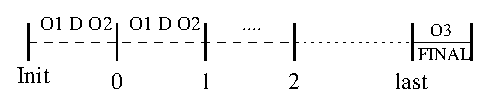
\includegraphics[scale=1.1]{scheduling.eps}
\end{center}
\caption{Observer and Dynamics scheduling\label{obsfigure}}
\end{figure}


In the Figure\ref{obsfigure}, O1,2,3 are \emph{Observer} components
and D represents one or more \emph{Dynamics} objects. Please note
that before the first protocol run a first \emph{Dynamics} and \emph{Observer}
run is performed (depicted in the interval between init and cycle
0). The snapshots taken by the \emph{Observer} objects are sent to
standard output and can be easily redirected to a file to be collected
for further work. Nevertheless, a developer can write \emph{Observer}
objects with a GUI or with database connection to store data directly
or whatever.


\subsection{The config file}
\label{configfile}

The config file is a plain ASCII text file, basically composed of
key-value pairs; the lines starting with \char`\"{}\#\char`\"{} character
are ignored (comments). The pairs are collected by a standard Java
\emph{java.util.Properties} object when the simulator starts using
for example the following command:\\


\texttt{\footnotesize \$> java -cp <class-path> peersim/cdsim/Simulator
config-file.txt}\\


Clearly the classpath is mandatory only if you haven't set it yet
in a global shell variable. Because of the spiritus of this tutorial,
we'll try to learn peersim and its basic components
using a by example metodology.


\subsection{Configuration example 1}

First of all, what we are going to do in this first experiment? 

We are going to impose a fixed P2P random topology composed by 50000
node network; the choosen protocol is \emph{Aggregation} (what is
aggregation? see section \ref{sec:Appendix-A-aggregation}) using
an average function. The values to be aggregated (averaged) at each
node are initialized using a linear distribution on the interval {[}0,
100{]}. Finally an \emph{Observer} monitors the averaging values.
Looks easy!!\\

\footnotesize
\begin{verbatim}
 1  # PEERSIM EXAMPLE 1
 2  # random.seed 1234567890
 3  simulation.cycles 30
 4  simulation.shuffle
 5 
 6  overlay.size 50000
 7  overlay.maxsize 100000
 8 
 9  protocol.0 peersim.core.IdleProtocol
 10 protocol.0.degree 20
 11
 12 protocol.1 example.aggregation.AverageFunction
 13 protocol.1.linkable 0
 14
 15 init.0 peersim.init.WireRegularRandom
 16 init.0.protocol 0
 17 init.0.degree 20
 18
 19 init.1 example.loadbalance.LinearDistributionInitializer
 20 init.1.protocol 1
 21 init.1.max 100
 22 init.1.min 1
 23
 24 observer.0 example.aggregation.AverageObserver
 25 observer.0.protocol 1
\end{verbatim}
\normalsize


Lets comment the code line by line. The first thing to node are the
key names: some of them are indexed and some other not (e.g. protocol.0.xxx
versus simulation.$<$parameter$>$). That means the unindexed keys refers
to static simulation elements, in fact the simulation itself is one
and the same holds for the P2P network: only one network! 

For the other simulation components you can think about the existance
of a dedicated array for each of their type (one for protocols, initailizer,
...); the \textsf{index} is the only reference to deal with them.
So the key for indexed components can be (informally) expressed as:
\\


\texttt{\footnotesize <init | protocol | observer | dynamics> . index\_number
{[}. <parameter\_name>{]}}~\\
{\footnotesize \par}

The final $<$parameter\_name$>$ is contained between {[}{]} to express
that it can be not present. This is the case when the element is declared.
For example, at \textbf{line 9}, the first protocol choosen comes to life;
the \textbf{key part} contains its type (or interface type) followed
by the index (always starting from 0, as in arrays) and \textbf{the
value} part contains the desired component class full package path
(you have to check the javadoc files or the source tree to discover
the correct package path). In the case of a component parameter declaration,
the \textbf{key part} contains the parameter name and the \textbf{value
part} is simply the value desired (usually an integer or a float).

At this point, should be clear that \textbf{from line 3 to line 7}
some global simulation properties are imposed; these are the total
number of simulation cycles and the overlay network size. The parameter
\texttt{simulation.shuffle} (\textbf{line} \textbf{4}) it is a little
different from what we have stated until now; it is used as a flag,
so it does not need a parameter. Its job is to shuffle the order in
which the nodes are visited in each cycle. The parameter \texttt{overlay.maxsize}
(\textbf{line7}) sets an upper bound on the network size, but in this
example it is useless (you can comment it out) and it's only present
for sake of completeness (will be useful next). 

From \textbf{line 9 to line 13}, two protocols are put in the arena.
The first one, peersim.core.IdleProtocol does nothing. It is useful
because of its ability to access to the topology, in fact it provides
neighbour links to each node. This feature is present because \emph{IdleProtocol}
is an implementation of the \emph{Linkable} interface. Next line declares
the graph degree. 

The second protocol (index 1: \texttt{protocol.1 aggregation.AverageFunction})
is the averaging version of aggregation. Its parameter (linkable)
is extremely important: it expresses the need to access the topology
using not this protocol itself (aggregation). This is due to the structure
of aggregation: it does not implement the \emph{Linkable} interface,
so it can't see the neighbor list by itself and it must use some other
protocol to do that. The value of parameter linkable is the index
of a \emph{Linkable} interface implementing protocol (\emph{IdleProtocol}
in the example). Clearly to know if a protocol can get access to the
topology directly, you have to check the documentation (or source
code!).

From \textbf{line 15 to line 22}, it's time to initialize all the
components previously declared. Again, the initialization components
are 2 and are indexed as usual. The first initializer 
\texttt{peersim.init.WireRegularRandom},
imposes a topology. The nodes using the declared protocol are linked
randomly to aechother to form a random graph having the specified
degree parameter. Please note that this degree declaration is exactly
the same of the previous (the one dedicated to the first protocol
creation). 

The second initializer task is to initialize the aggregation function
value-field to be averaged. The initialization values follows a linear
distribution fashion. The parameters declared are three: \texttt{protocol},
\texttt{max}, \texttt{min}. Respectively, their meaning is:

\begin{itemize}
\item a protocol to point to: the initializer needs a reference (index)
to a protocol extending \emph{aggregation.AbstractFunction} Class
to get access to the value to be aggregated (averaged); it is clear
that this protocol must be \emph{aggregation.AverageFunction} (index
1);
\item the maximum value in the linear distribution; 
\item the minimum value in the linear distribution 
\end{itemize}
Finally at \textbf{line 24,25} the last component is declared: 
\texttt{aggregation.average Observer}.
Its only parameter used is protocol and clearly refers to an \emph{aggregation.
AverageFunction} protocol type, so the parameter value is index 1
(in fact: \texttt{protocol.1 aggregation.AverageFunction}). 

Now you can try the example writing on a console the following line:\\


\texttt{\footnotesize \$> java -cp <class-path> peersim/cdsim/Simulator
example1.txt}~\\
{\footnotesize \par}

The classpath is mandatory only if the used system has not peersim
classes in the shell CLASSPATH environment variable. To get the exact
output that will follow, the reader should uncomment the parameter
at \textbf{line 2}:\\


\texttt{\footnotesize random.seed 1234567890}~\\
{\footnotesize \par}

on top of the configuration file. This parameter is very useful to
replicate exactly the experiments results based on (pseudo) random
behaviour. The experiment output is (some initialization string may
be different):\\

\tiny
\begin{verbatim}
 Simulator: loading configuration
 ConfigProperties: File example/config-example1.txt loaded.
 Simulator: starting experiment 0
 Simulator: resetting overlay network
 Network: no node defined, using GeneralNode
 Simulator: running initializers
 - Running initializer 0: class peersim.init.WireRegularRandom
 - Running initializer 1: class example.loadbalance.LinearDistributionInitializer
 Simulator: loaded observers [observer.0]
 Simulator: loaded modifiers []
 Simulator: starting simulation
 observer.0 0 28.57969570575493 1.0 50.49999999999998 100.0 1.0 50000 50000
 Simulator: cycle 0 done
 observer.0 1 15.744375112466432 0.5508937280006126 50.500000000000185 99.64260285205704 1.993979879597592 50000 50000
 Simulator: cycle 1 done
 observer.0 2 8.77307045667709 0.3069686446980087 50.50000000000009 86.06868887377748 11.048700974019479 50000 50000
 Simulator: cycle 2 done
 observer.0 3 4.909681896225926 0.17178915922597776 50.499999999999794 74.03587220181905 22.769780085543115 50000 50000
 Simulator: cycle 3 done
 observer.0 4 2.7403309556342257 0.09588383948687113 50.500000000000426 65.43171163227953 33.427798365537626 50000 50000
 Simulator: cycle 4 done
 observer.0 5 1.538286672869342 0.053824459459153234 50.49999999999973 59.82515640226745 42.62594413722992 50000 50000
 Simulator: cycle 5 done
 observer.0 6 0.866397905938638 0.03031515502679675 50.50000000000007 55.26130498088358 45.94325388089578 50000 50000
 Simulator: cycle 6 done
 observer.0 7 0.485544546348093 0.016989143318636584 50.4999999999996 53.34350686753126 47.92146780934889 50000 50000
 Simulator: cycle 7 done
 observer.0 8 0.27325943590085566 0.009561313693267594 50.499999999999936 51.953084686348944 49.100818456230826 50000 50000
 Simulator: cycle 8 done
 observer.0 9 0.15407802503043988 0.005391170942362905 50.499999999999545 51.464657035213264 49.43879802069546 50000 50000
 Simulator: cycle 9 done
 observer.0 10 0.08620333588583261 0.0030162440067013846 50.500000000000156 51.099961126584006 49.98131655222747 50000 50000
 Simulator: cycle 10 done
 observer.0 11 0.04848730705794467 0.0016965648464962858 50.4999999999997 50.816956855036466 50.22577832539035 50000 50000
 Simulator: cycle 11 done
 observer.0 12 0.027214744249562235 9.522405182250473E-4 50.499999999999524 50.65301253758219 50.29955826845794 50000 50000
 Simulator: cycle 12 done
 observer.0 13 0.015246845383671713 5.334852246380476E-4 50.50000000000032 50.59479421528527 50.38736504947625 50000 50000
 Simulator: cycle 13 done
 observer.0 14 0.008587160488627146 3.004636780264248E-4 50.499999999999815 50.543660258997136 50.44122418780829 50000 50000
 Simulator: cycle 14 done
 observer.0 15 0.004850437249792671 1.697161964119851E-4 50.50000000000037 50.52544970665122 50.46753516145482 50000 50000
 Simulator: cycle 15 done
 observer.0 16 0.0027428141606463717 9.59707265215587E-5 50.50000000000047 50.515509548126744 50.48203242786418 50000 50000
 Simulator: cycle 16 done
 observer.0 17 0.001550607390364058 5.4255559832703925E-5 50.4999999999997 50.50982384430303 50.49003444731606 50000 50000
 Simulator: cycle 17 done
 observer.0 18 8.746858998689715E-4 3.0605150904137896E-5 50.5000000000003 50.50564226243819 50.495105203016905 50000 50000
 Simulator: cycle 18 done
\end{verbatim}
\normalsize

The observer component produces many numbers, but looking at the 6th and
7th data columns (respectively the maximum of averages and the minimum
of averages) it's easy to see how the variance decreases very quickly.
At cicle 12 (look at the underlined data), quite all the nodes has
a very good approximation of the real average (50). Try to experiment
with different numbers and then to change the init distribution (e.g.:
using \texttt{aggregation.Peak DistributionInitializer}) and / or the
protocol stack (put \emph{Newscast} or \emph{SCAMP} instead of 
\emph{IdleProtocol}).


\subsection{Configuration example 2}

This second example is an improved version of the first one. What's
new? Now the aggregation protocol runs on top of Newscast and it's
easy to switch to the peak distribution (comment 4 lines and uncomment
2 lines). Moreover, there is a Dynamics object that changes the network
size (it shrinks it by cutting out 500 nodes each time). \\

\footnotesize
\begin{verbatim}
 1  simulation.cycles 30
 2  simulation.shuffle
 3
 4  overlay.size 50000
 5  overlay.maxsize 200000
 6
 7  protocol.0 example.newscast.SimpleNewscast
 8  protocol.0.cache 20
 9
 10 protocol.1 example.aggregation.AverageFunction
 11 protocol.1.linkable 0
 12
 13 init.0 peersim.init.WireRegularRandom
 14 init.0.protocol 0
 15 init.0.degree 20
 16 
 17 #init.1 example.aggregation.PeakDistributionInitializer
 18 #init.1.value 1
 19 init.1 example.loadbalance.LinearDistributionInitializer
 20 init.1.protocol 1
 21 init.1.max 100
 22 init.1.min 1
 23
 24 observer.0 example.aggregation.AverageObserver
 25 observer.0.protocol 1
 26
 27 dynamics.0 peersim.dynamics.GrowingNetwork
 28 dynamics.0.add -500
 29 dynamics.0.minsize 4000
 30 dynamics.0.from 5
 31 dynamics.0.until 10
\end{verbatim}
\normalsize

The global parameters are the same as in the previous example; only
new additions are discussed below. At \textbf{line 7-8} there is the
\emph{Newscast} (what is newscast? see section \ref{sec:Appendix-B-newscast}) 
component declaration with its
only parameter cache (please note: cache size should be at least as
large as network degree size). At \textbf{line 17-18} there is a different
distribution type: \texttt{aggregation.PeakDistribution Initializer},
but it's inactive. To switch it on, simply delete the preceeding simbol
\char`\"{}\#\char`\"{} and comment out the following 4 lines. The
peak distribution initializes all nodes except one with 0 value and
the node left takes the value declared in parameter value.

From \textbf{line 27 to 32} is present the last new component: 
\texttt{dynamics.0
peersim.dynamics.GrowingNetwork}. As stated previously, a \emph{Dynamics}
interface implementing object is able to change some other object
properties; the change can be performed at each simulation cycle (default
behaviour) or using a more sophisticated idea. The object choosen
in the example deletes 500 nodes from the net at each time (well,
it is not completely correct to talk about deletion in the peersim
vision, in fact the \emph{Linkable} interface does not support node
deletion from the overlay; so it's better to think about \char`\"{}unlinking\char`\"{}
nodes from the overlay). The parameters \texttt{add}, \texttt{minsize},
\texttt{from} and \texttt{until} have respectively the following meaning:

\begin{itemize}
\item adds the specified number of nodes (if negative subracts);
\item the minimum size ir referred to the overlay: it can't be less than
what's stated here;
\item the cycle number from which the \emph{Dynamics} object can start running;
\item the cycle number until which the \emph{Dynamics} object can run.
\end{itemize}
Other parameters are avaiable, please check the source or the JavaDoc.

It's interesting to note that not all the parameters associated to
a \emph{Dynamics} component can be found in the \emph{Dynamics} itself
source code (or documentation); this is due to the Simulator class
behaviour. When it creates the \emph{Dynamics} object instances (this
hold also for \emph{Initializer} and \emph{Observer} objects), it
wraps them in a \emph{Scheduler} class object: this is the class where
some parameters (such as \texttt{step}, \texttt{from}, \texttt{until})
are actually defined.

\subsection{Advanced configuration features}

Thanks to the presence of the Java Expression Parser (since release
0.2), the configuaration
file can handle many types of \textbf{expressions}, such as boolean 
expressions, 
common
mathematical functions and well known predifined constants (e.g.: $\pi$ 
and
$e$); for an exhaustive feature list check the Java Expression Parser
web page (\url{http://www.singularsys.com/jep/index.html}).\\
Expresions can be used anywhere instead of numeric values, as follows:

\begin{verbatim}
MAG 2
SIZE 2^MAG
\end{verbatim}

the variable SIZE will be automagically evaluated in number 4.\\
Multiple expressions can be written in a tree-like fashion and they'll
be evaluated recursively (the cpu conscious users have to know that 
no optimizations are performed and the same expression may be evaluated
many times) as in the following code sample:

\begin{verbatim}
A B+C
B D+E
C E+F
D 1
E F
F 2
\end{verbatim}

The evaluation will produce: A=7, B=3, C=4, D=1, E=2 and F=2.\\
\\
Recursive definitions are not allowed and a simple trick is used to 
avoid them: if the recursion depth is grater than a configurable 
threshold parameter (set at 100 by default) an error message is
printed and the simulator stops.\\
\\
For any kind of simulator object (means Dynamics, Observer, Protocol),
it is possible to specify an ordering scheme and to specify an arbitrary 
name to multiple instances of a given entity. The object prefixes are
not limited to numerical indexes, but they can be expressed by any 
string, as follows:

\begin{verbatim}
observer.conn ConnectivityObserver
observer.0 Class1
observer.1 Class2
\end{verbatim}

The order is lexicographically, but can be explicitly rearranged
giving an object name list separated  by any non-word character
(non alphanumeric or underscore):

\begin{verbatim}
order.observer 2,conn,0
\end{verbatim}

If not all names appear in the list,
then the vacant objects will follow the default alphabetical order.
For example:

\begin{verbatim}
order.observer 2
\end{verbatim}

will produce the following order:

\begin{center}
$\langle$ \texttt{observer.2} ; \texttt{observer.0} ; \texttt{observer.conn} $\rangle$
\end{center}

Another available feature is the chance to exclude items from the
list. To obtain this effect type:

\begin{verbatim}
include.observer conn 2
\end{verbatim}

This will return \texttt{observer.conn} and \texttt{observer.2} in this 
exact order. If the list is empty, then an empty ordering array will be
generated; means that, in this case, no observer will run. Note that 
\texttt{include} is stronger than \texttt{order}
infact if the former is defined, then the latter is ignored.
 
\subsubsection{A concrete example}

To have a pratical idea about how to use these new features, the following
example is presented; it is a modified example2 version.

\footnotesize
\begin{verbatim}

1 #random.seed 1234567890
2 simulation.cycles 30
3 simulation.shuffle
4
5 # Imposes the correct protocol running order:
6 order.protocol ncast,avgagr
7
8 overlay.size 50000
9 overlay.maxsize 200000
10 
11 protocol.ncast example.newscast.SimpleNewscast
12 protocol.ncast.cache 20
13
14 protocol.avgagr example.aggregation.AverageFunction
15 protocol.avgagr.linkable ncast
16
17 init.wrr peersim.dynamics.WireRegularRandom
18 init.wrr.protocol ncast
19 init.wrr.degree 20
20
21 # UNCOMMENT THE FOLLOWING LINES TO GET A PEAK DISTRIBUTION
22 #init.pkdistrib example.aggregation.PeakDistributionInitializer
23 #init.pkdistrib.value 10000
24 #init.pkdistrib.protocol avgagr
25
26 # UNCOMMENT THE FOLLOWING LINES TO GET A LINEAR DISTRIBUTION
27 init.ldistrib example.loadbalance.LinearDistributionInitializer
28 init.ldistrib.protocol avgagr
29 init.ldistrib.max 100
30 init.ldistrib.min 1
31
32 observer.avgobs example.aggregation.AverageObserver
33 observer.avgobs.protocol avgagr
34
35 dynamics.grnetwork peersim.dynamics.GrowingNetwork
36 dynamics.grnetwork.add -500
37 dynamics.grnetwork.minsize 4000
38 dynamics.grnetwork.from 5
39 dynamics.grnetwork.until 10
\end{verbatim}
\normalsize

In this configuration file, the protocol indexes are no more used; 
but the same holds for each kind of object. A symbol string that
summarize the original class name is used instead of an index number.
Bacause of the choosen protocol symbol names (\texttt{ncast} and 
\texttt{avgagr}),
it is necessary to impose a different running order scheme to let
newscast run first using (at \textbf{line 6}):

\begin{verbatim}
order.protocol ncast,avgagr
\end{verbatim}

\section{Writing a new protocol}

This section covers the description of how to write a new protocol. 


\subsection{Which kind of protocol?}

The protocol we are going to develop is a simple load balancing algorithm.
It works as follows. The state of a node is composed of two values:
the local load and the quota; the second one is the amount of \char`\"{}load\char`\"{}
the node is allowed to transfer at each cycle. The quota is necessary
in order to make real load balancing, otherwise it would be simply
averaging. Every node contacts the most \textbf{distant} neighbor
in its local view and then exchanges at maximum the quota value. The
concept of \char`\"{}distance\char`\"{} is expressed in terms of maximally
different load from the current node local load. Comparing the distance
to the actual node load, the protocol chooses to perform a load balance
step using a push or pull approach.

After each cycle, the quota value is restored to allow further computation.
The protocol does not care about topology management and relies on
other components to get access to this feature (e.g.: \emph{Newscast},
\emph{IdleProtocol}). 


\subsection{Needed components}

Now we have a general idea on what we want to code and it's time to
adapt it to the peersim framework. Writing a the protocol class itselt,
it is usually not sufficient. Some companion components are required.
For example, to restore the quota value for each node at the end of
each cycle, a specific \emph{Dynamics} object is required. Peersim
is basically a collection of interchangeable components, so the development
of new stuff should have \textbf{modularity} in mind and should maximize
code reuse. To acheive this, the following classes are proposed:

\begin{itemize}
\item protocol class itself: it is built on (extends) aggregation.AbstractFunction;
this strategy permits the reuse of the aggregation protocol \char`\"{}value\char`\"{}
field and related methods to store the load value. Sharing the same
interface as aggregation, many other components can be used toghether
with the load balancing protocol, such as the initializers classes. 
\item Dynamics component: it is necessary to restore the quota value at
each node at the end of each cycle (as previously stated). This object
is quite straighforward: it simply implements the only one method
the interface \emph{Dynamics} declares, invoking the protected protocol
method \emph{resetQuota()}. 
\item Initializer and Observer components: are not needed!
The aggregation initializers can be used directly. Also the aggregation
observers can be used (the \emph{aggregation.AverageObserver} in particular).
In addition a new observer object can be written to monitor the quota
parameter and thus the amount of traffic performed in the overlay.
\end{itemize}
To give the reader an idea about the actual code to write, the following
subsections are presented, in which the author put comments and explanations
in the way of the class code itself.

\footnotesize
\begin{verbatim}
 package loadbalance;
 
 import peersim.util.CommonRandom;
 import aggregation.AbstractFunction;
 import peersim.config.Configuration;
 import peersim.core.*;
 
 public class BasicBalance extends AbstractFunction {
 // Fields:
 // allowed config file parameter
 public static final String PAR_QUOTA = "quota";
 // original quota value taken from configuration 
 private final double quota_value; 
 
 protected double quota; // current cycle quota
 
 // Constructor:
 public BasicBalance(String prefix, Object obj) {
     super(prefix, obj);
     // get quota value from the config file. Default 1.
     quota_value = (double)(Configuration.getInt(prefix+"."+PAR_QUOTA, 1));
     quota = quota_value;
 }
\end{verbatim}
\normalsize


It's simply standard Java code until now; the package loadbalance
and the needed classes are declared. Extending \emph{AbstractFunction},
we implements \emph{CDProtocol} and \emph{Protocol} interfaces automagically,
but we need to override the previously defined methods to avoid using
the \emph{AbstractFunction} implementation.

In the constructor signature, two parameters are present; the first
one is a string corrisponding to the configuration file protocol key
(e.g.: protocol.1 in the \emph{LoadBalance} protocol case), the second
one is the protocol id index casted in a \emph{Object} type. These
parameters are used in the superclass (\emph{aggregation.AbstractFunction})
to connect this class to a Likable implementing protocol class. As
an example, the \emph{aggregation.AbstractFunction} constructor class
it's presented:\\

\footnotesize
\begin{verbatim}
public AbstractFunction(String prefix, Object obj) {
     int protocolId = ((Integer) obj).intValue();
     int link = Configuration.getPid(prefix+"."+PAR_CONN);
     Protocols.setLink(protocolId, link);
 }
\end{verbatim}
\normalsize


The special method \emph{getPid()} is present to retrive a protocol
identifier; the configuration property (input) is converted into a 
numeric protocol id. The property can be any string and it's mapped to
an integer according to the particular ordering scheme applied to the
protocol names.\\
The static class \emph{Protocols} collects protocol id-s of the protocols
from which instances of this class get neighborhood info. The \emph{protocolID}
variable represents the current class and the \emph{link} variable
index is the \emph{Linkable} enabled protocol stated in the configuration
file (\texttt{linkable} parameter).\\

\footnotesize
\begin{verbatim}
 // Resets the quota. 
 protected void resetQuota() {
     this.quota = quota_value;
 }
\end{verbatim}
\normalsize

The \emph{resetQuota()} method is called by the dynamics object at
the cycle end. Clearly a suitable dynamics entry should be present
in the configuration file (such as: \texttt{dynamics.0 loadbalance.ResetQuota}
and \texttt{dynamics.0. protocol protocol-index}). This method is not
mandatory, but it's much more software engineering oriented then a
dirty variable access performed by the dynamics object.\\

\footnotesize
\begin{verbatim}
 // Implements the Protocol interface
 public Object clone() throws CloneNotSupportedException {
     BasicBalance af = (BasicBalance)super.clone();
     return af;
 }
 
 // Implements CDProtocol interface
 public void nextCycle( Node node, int protocolID ) {
     int linkableID = Protocols.getLink(protocolID);
     Linkable linkable = (Linkable) node.getProtocol( linkableID );
     if (this.quota == 0) {
         return; // skip this node
     }    
     // this takes the most distant neighbor based on local load
     BasicBalance neighbor = null;
     double maxdiff = 0;
     for(int i = 0; i < linkable.degree() ; ++i)
     {
         Node peer = linkable.getNeighbor(i);
         // The selected peer could be inactive
         if(!peer.isUp()) continue; 
         BasicBalance n = (BasicBalance)peer.getProtocol(protocolID);
         if(n.quota!=1.0) continue;
         double d = Math.abs(value-n.value);
         if( d > maxdiff )
         {
             neighbor = n;
             maxdiff = d;
         }
     }
     if( neighbor == null ) {
         return;
     }
                 
     doTransfer(neighbor);
 }
\end{verbatim}
\normalsize


The first method is required by the Protocol interface and basically
calls the ancestor cloning method. So, nothing special here.

The second one is required by \emph{CDProtocol} interface. It is the
action performed by the protocol. The arguments represents a reference
to the node itself (the node on which the simulator is invoking the
\emph{nextCycle()} method) and the index protocol identifier (\emph{BasicBalance}
in this case). First it has to get a reference (in indexed form) to
the \emph{Linkable} interface enabled protocol in the node protocol
stack; as a remind, something implementing the \emph{Linkable} interface,
is an entity capable of accessing to the topology. Having this linkable
reference we can access to the real \emph{Linkable} interface
implementation with: \\


\texttt{\footnotesize Linkable linkable = (Linkable) node.getProtocol(
linkableID );}~\\
{\footnotesize \par}

If the local quota is equal to 0, means that the node we have already
spent its amount of network traffic, so it returns.

To get the most distant node from the current one, a for loops on
all neighbor node load value; the number of neighbor is equal to the
node degree (aceesible thanks to \emph{Linkable} interface). To pick
a node having a the \emph{Linkable} access:\\


\texttt{\footnotesize Node peer = linkable.getNeighbor(i);} \\


and from this obtained \emph{Node} interface reference it is possible
to get the protocol interface we are interested in (\emph{BasicBalance}):\\


\texttt{\footnotesize BasicBalance n = (BasicBalance)peer.getProtocol(protocolID);}
\\


When the protocol finds a suitable neighbor, it performs a load balancing
step invoking the \emph{doTransfer()} method.\\

\footnotesize
\begin{verbatim}
 // Performs the actual load exchange selecting to make a PUSH or PULL approach.
 // It affects the involved nodes quota. 
 protected void doTransfer(BasicBalance neighbor) {
     double a1 = this.value;
     double a2 = neighbor.value;
     double maxTrans = Math.abs((a1-a2)/2);
     double trans = Math.min(maxTrans,quota);
     trans = Math.min(trans, neighbor.quota);
 
     if( a1 <= a2 ) // PULL
     {
         a1+=trans;
         a2-=trans;
     }
     else // PUSH
     {
         a1-=trans;
         a2+=trans;
     }
     
     this.value = a1;
     this.quota -= trans;
     neighbor.value = a2;
     neighbor.quota -= trans; 
 }
\end{verbatim}
\normalsize


The last method takes as parameter a reference to the picked neighbor.
This is the place where it's time to decide to perform a pull or a
push load balancing approach. To make this choice the local load value
is compared with the neighbor load value. In case of a push choice,
the local value is increased and the other node value is decresed;
in the other case (pull) the exact opposite holds. The \emph{maxTrans}
variable is the absolute amount of \char`\"{}load\char`\"{} to transfer
to reach the balance between the two involved nodes; because of the
quota upper bound on the transfers at each cycle, the algorithm chooses
the minimum between the quota itself and the aimed \emph{maxTrans}
amount. The quota value is decreased by the same amount at both nodes.


\subsection{Load balancing dynamics class code}

\footnotesize
\begin{verbatim}
 package loadbalance;
 
 import peersim.config.*;
 import peersim.core.*;
 import peersim.dynamics.Dynamics;
 
 public class ResetQuota implements Dynamics {
 // Fields:
 public static final String PAR_VALUE = "value";
 
 public static final String PAR_PROT = "protocol";
 
 private final double value;
 private final int protocolID;
 
 // Constructor:
 public ResetQuota(String prefix)
 {
     value = Configuration.getDouble(prefix+"."+PAR_VALUE);
     protocolID = Configuration.getPid(prefix+"."+PAR_PROT);
 }
 
 // Dynamics interface method:
 public void modify() {
     for(int i=0; i < OverlayNetwork.size(); ++i)
     {
         ((BasicBalance)OverlayNetwork.get(i).getProtocol(protocolID)).resetQuota();
     }
   }
 }
\end{verbatim}
\normalsize

The code is very compact because the \emph{Dynamics} interface itself
is very simple: only the \emph{modify()} method. The costructor takes
care of initializing the configuration file parameters (respectively:
the reset value and the protocol identifier to deal with). The \emph{modify()}
method makes use of network global knowledge: it invokes the \emph{resetQuota()}
method on all the \emph{OverlayNetwork} object elements (it's a static
object avaiable everywhere in the simulator environment; you can think
about it as an array). It is clear that the simulator has global knowledge,
but it is up to the protocol developer to make use or not of this
facility according to the consistency of the simulation itself. 


\subsection{Implementing the Linkable interface}

In this howto there are a lot of references about the \emph{Linkable}
interface and about its importance, so for the sake of completeness,
it's time to give a look at how to implement it in brief. It's interesting
to node that this interface should be implemented by low level or
by topology management protocols and not by a higher level protocol
such as a load balancing one. The reason to discurage the implementation
is the risk to affect modularity. At least, the reader should consider
the ability to switch off the built in \emph{Linkable} interface and
to use an external protocol facility instead.

The interface defines five methods: \emph{degree()}, \emph{getNeighbor()},
\emph{addNeighbor()}, \emph{contains()}, \emph{pack()}. These methods
are not usually invoked by the protocol itself (except for \emph{getNeighbor()}
), but by an \emph{Initializer} object instead. Please note that there
is no way to remove nodes from the overlay; the only chance to get
a similar effect, is to disable a peer accessing to the \emph{peersim.core.Fallible}
interface (extended by the \emph{Node} interface) and setting one
of the available node states (\emph{peersim.core.Fallible.OK | DEAD | 
MALICIUS | DOWN}). 

A feasible implementation could be the following. First of all, the
class (e.g.: \emph{BasicBalance}) needs a structure to represent the
neighbor view: an \emph{ArrayList} structure it's fine.\\

\footnotesize
\begin{verbatim}
 protected ArrayList nView = null;
 // Constructor:
 
 public BasicBalance(String prefix, Object obj) {
     ...
     nView = new ArrayList();
     ...
 }
 // Linkable interface implementation methods:
 public int degree() {
     return nView.size();
 }
 
 public Node getNeighbor(int i) {
     return (Node)nView.get(i);
 } 
 
 public boolean addNeighbor(Node n) {
     if (!contains(n)) {
         nView.add(n);
         return true;
     }
     else {return false;}
 }
 
 public boolean contains(Node n) {
     return nView.contains(n);
 }
 
 public void pack() { ; } // unused!
\end{verbatim}
\normalsize

Again the code is quite straightforward. All the elements inside the
view are \emph{Node} class (interface) types. All methods are simple
functions built upon the \emph{ArrayList} structure. The last method
is included in the interface description with the aim to provide a
view size compression facility, but it's usually not implemented (the
size of each view is tipically quite small).


\section{A second new protocol}

This new protocol is an extensions of the previous one. The general
core is quite the same, but the algorithm uses the global load average
value instead of the most distant neighbor load value. To calculate
the global load average, a little trick is used; it would be possible
to calculate this value using aggregation, but we can \textbf{simulate}
the aggregation effect (alias calculating the average load) by running
a static method with global knowledge once. This method will initialize
a global variable available to all nodes. 

This protocol is targeted to gain advantage from the newscast protocol
features; when a node reaches the global load value (average), it
switches to a DOWN state. In this way, the node exits from the overlay
and the newscast protocol no more cares about it. The effect is that
the topology shrinks as soon as the nodes reach the average load.
\\

\footnotesize
\begin{verbatim}
 package loadbalance;
 
 import peersim.util.CommonRandom;
 import aggregation.AbstractFunction;
 import peersim.core.*;
 
 public class AvgBalance extends BasicBalance {
 
     public static double average = 0.0;
     public static boolean avg_done = false;
     
     // Costructor:
     public AvgBalance(String prefix, Object obj) {
         super(prefix, obj);
     }
 
        // Method to simulate average function aggregation
     private static void calculateAVG(int protocolID) {
         int len = OverlayNetwork.size();
         double sum = 0.0;
         for (int i = 0; i < len; i++) {
             AvgBalance protocol = (AvgBalance)OverlayNetwork.get(i).getProtocol(protocolID);
             double value = protocol.getValue();
             sum += value;
         }
         average = sum / len;
         avg_done = true;
     }
\end{verbatim}
\normalsize


The first part is straightforward. Two global variables are defined:
average, and avg\_done; the second is a flag used to be sure not to
perform the calculation more than once. A different and much more
elegant approach is to define the average calculation method inside
a static constructor, but this solution is \textbf{wrong}! When the
node protocol objects are created, the load distribution is not defined
yet, so the global average result will be 0.

The function \emph{calculateAVG()} simulates the average aggregation
behaviour. It makes use of global knowledge, looping on each overlay
node. \\


\texttt{\footnotesize protected static void suspend( Node node ) \{}{\footnotesize \par}

\texttt{\footnotesize node.setFailState(Fallible.DOWN); }{\footnotesize \par}

\texttt{\footnotesize \}}{\footnotesize \par}

This is the utility function to exit from the topology; simply sets
a node state from \emph{Fallible} interface.\\

\footnotesize
\begin{verbatim}
 // CDProtocol Interface implementation. Overrides the BasicBalance implementation:
     public void nextCycle( Node node, int protocolID ) {
         // Do that only once
         if (avg_done == false) {
             calculateAVG(protocolID);
             System.out.println("AVG only once "+average);
         }
    
         if( Math.abs(value-average) < 1 ) {
             AvgBalance.suspend(node); // switch off node
             return;
            }
     
         if (quota == 0 ) return;
     
         Node n = null;
         if (value < average ) {
             n = getOverloadedPeer(node, protocolID);
             if (n != null) { doTransfer((AvgBalance)n.getProtocol(protocolID)); } 
         }
         else {
             n = getUnderloadedPeer(node, protocolID);
             if (n != null) { doTransfer((AvgBalance)n.getProtocol(protocolID)); } 
         } 
     
         if( Math.abs(value-average) < 1 ) AvgBalance.suspend(node);
         if (n != null) {
             if( Math.abs(((AvgBalance)n.getProtocol(protocolID)).value-average) < 1 ) 
	            AvgBalance.suspend(n);
         }
     }
\end{verbatim}
\normalsize

Method \emph{nextCycle()} is the protocol algorithm core. It first
checks for the average calculation: if the flag is not set, it performs
the computation.

If the difference between the current and the average load is less
then 1 (the fixed quota value per cycle) the node is suspended and
thus exits from the topology defined by the newscast protocol; moreover,
if the quota has been already spent, it returns. The protocol then
checks if the local value is less or grater then the average and respectively
get the most loaded or the least loaded neighbor and exchange.\\

\footnotesize
\begin{verbatim}
 private Node getOverloadedPeer(Node node, int protocolID) {
         int linkableID = Protocols.getLink(protocolID);
         Linkable linkable = (Linkable) node.getProtocol( linkableID );
     
         AvgBalance neighbor=null;
         Node neighborNode = null;
         double maxdiff = 0.0;
         for(int i = 0; i < linkable.degree(); ++i) {
             Node peer = linkable.getNeighbor(i); 
             if(!peer.isUp()) continue;
             AvgBalance n = (AvgBalance)peer.getProtocol(protocolID);
             if(n.quota==0) continue;
             if(value >= average && n.value >= average) continue;
             if(value <= average && n.value <= average) continue;
             double d = Math.abs(value-n.value); 
             if( d > maxdiff ) {
                 neighbor = n;
                 neighborNode = peer;
                 maxdiff = d;
             }
         }
         return neighborNode;
     } 
 
     private Node getUnderloadedPeer(Node node, int protocolID) {
         int linkableID = Protocols.getLink(protocolID);
         Linkable linkable = (Linkable) node.getProtocol( linkableID );
     
         AvgBalance neighbor=null;
         Node neighborNode = null;
         double maxdiff = 0.0;
         for(int i = 0; i < linkable.degree(); ++i) {
             Node peer = linkable.getNeighbor(i);
             if(!peer.isUp()) continue;
             AvgBalance n = (AvgBalance)peer.getProtocol(protocolID);
             if(n.quota==0) continue;
             if(value >= average && n.value >= average) continue;
             if(value <= average && n.value <= average) continue;
             double d = Math.abs(value-n.value); 
             if( d < maxdiff ) {
                 neighbor = n;
                 neighborNode = peer;
                 maxdiff = d;
             }
         }
         return neighborNode;
     } 
 } // end of class
\end{verbatim}
\normalsize


The methods to get the the most loaded or the least loaded neighbor
are straighforward and very similar, but are shown for completeness.


\section{Evaluating the protocols}

The performance about load variance reduction can be analyzed with
an \emph{aggregation.Average Observer} or a \emph{loadbalance.LBObserver}
(they are very similar), but don't expect huge differences. In fact,
from this point of view, the two protocols have nearly an identical
performance, no matter whatever distribution you are using. The 
\emph{AVGBalance}
protocol improvement over the \emph{BasicBalance} one is about the
acheived overall load transfer. The \emph{AVGBalance} amount of transfer
is minimal and it is pratically the same of the theoretical minimal
amount of transfer needed to solve the problem 
(more about this: \url{http://www.cs.unibo.it/bison/publications/modular-p2p.pdf}). 

The \emph{Observer} class code to inspect the load transfer amount
is the following. \\

\footnotesize
\begin{verbatim}
 package loadbalance;
 
 import peersim.core.*;
 import peersim.reports.*;
 import peersim.config.*;
 import peersim.util.IncrementalStats;
 
 public class QuotaObserver implements Observer {
 
 public static final String PAR_PROT = "protocol";
 private final String name;   
 private final int pid;   // protocol id to monitor
 private IncrementalStats stats;   // object to compute statistics
 
 // Constructor:
 public QuotaObserver(String name) {
     this.name = name;
     pid = Configuration.getPid(name + "." + PAR_PROT);
     stats = new IncrementalStats();
 }
 
 // Observer interface implementation:
 public boolean analyze() {
     for (int i = 0; i < OverlayNetwork.size(); i++) {
         BasicBalance protocol =  (BasicBalance) OverlayNetwork.get(i).getProtocol(pid);
         stats.add( protocol.quota );
     }
     System.out.println(name+": "+stats);
     return false;
 }
 
 } // end of class
\end{verbatim}
\normalsize


The idea is very simple: at each simulation cycle it collects all
node values about quota and print statistics on the console.


\section{\label{sec:Appendix-A-aggregation}A few words about
Aggregation}

It is a very fast epidemic-style protocol targeted to compute a particular
function (e.g.: average, max, min, ...) on a numeric value holded
at each network node. In order to work, every node needs access to
its neighbor list view on the overlay network; no particular requirements
about the topology management protocol are imposed. In the case of
avaraging function, a generic method \emph{updateState(a, b)} returns
(a+b)/2, where a and b are values at (respectively) node a and node
b. This kind of computation is performed by each node at each simulation
cycle.

The global average is not affected, but the variance over all the
estimates decreses very fast in a few cycles (the convergence rate
is exponential and it does not care about the network size). The aggregation
protocol is also very robust in case of nede failures. 

Suggested readings: project BISON publication page \url{http://www.cs.unibo.it/bison/pub.shtml}.


\section{\label{sec:Appendix-B-newscast}A few words about Newscast}

Newscast is an epidemic content distribution and topology management
protocol. Every peer in the system has a partial view knowledge about
the topology which is modeled as a fixed size (c) set of node descriptors.
Each descriptor is a tuple consisting of a peer address and a timestamp
recording the time when the descriptor was created.

Each node updates its state by choosing a random neighbor and exchanging
with it the view. The exchanging process merges the two involved peer
partial view, keeping the c freshest descriptors. in this manner,
old information (descriptor) are automagically removed from the system
as time goes on. This process allows the protocol to repair the overlay
topology removing dead links with minimum effort and this is a great
feature for a highly dynamic oriented system where nodes join and
leave continously. 

The protocol relies on the timestamps, but it doesn't need synchronized
clocks: timestamps have to be only mutually consistent. To acheive
this, a simple time normalization of the received descriptors is performed.
So time precision is not critical at all. 

The emergent topology from newscast topology management has a very
low diameter and it is very close to a random graph with (out) degree
c. Suggested readings: "Large-Scale Newscast Computing on the Internet" \url{http://citeseer.nj.nec.com/jelasity02largescale.html}.

\end{document}
